\documentclass{article}

% NeurIPS 2024 template, preprint mode (single-column, author info visible).
\PassOptionsToPackage{numbers, compress}{natbib}
\usepackage[preprint]{neurips_2024}

\usepackage[utf8]{inputenc}
\usepackage[T1]{fontenc}
\usepackage{hyperref}
\usepackage{url}
\usepackage{booktabs}
\usepackage{amsfonts}
\usepackage{amsmath}
\usepackage{amssymb}
\usepackage{nicefrac}
\usepackage{microtype}
\usepackage{xcolor}
\usepackage{graphicx}
\usepackage{listings}
\usepackage{enumitem}
\usepackage{multirow}
\usepackage[ruled,linesnumbered]{algorithm2e}

% --- Placeholders for in-progress experimental numbers ---
% \todo{...} renders as a yellow-tinted in-line note we can search for later.
\definecolor{todoyellow}{HTML}{FFF4C2}
\newcommand{\todo}[1]{%
  \par\smallskip\noindent
  \fcolorbox{black!30}{todoyellow}{%
    \parbox{\dimexpr\linewidth-2\fboxsep-2\fboxrule\relax}{%
      \textbf{[TODO]}~#1%
    }%
  }\par\smallskip%
}

% Inline-friendly variant for short placeholders inside running prose / tables.
\newcommand{\itodo}[1]{\textcolor{red!75!black}{\textbf{[TODO:}~#1\textbf{]}}}

% --- Code / inline command shorthand ---
\newcommand{\code}[1]{\texttt{#1}}

\title{Asynchronous Compiler-Supervised Decoding for Code Generation}

% Single author for the course submission.
\author{%
  Leo Wang\thanks{Code and live demo:
    \href{https://github.com/leobwang/soundcode}{\code{github.com/leobwang/soundcode}};
    \href{https://soundcode-demo.psixyzt.com}{\code{soundcode-demo.psixyzt.com}}.}\\
  Department of Computer Science\\
  University of Chicago\\
  \texttt{psixyzt@gmail.com}\\
}

\begin{document}

\maketitle

\begin{abstract}
Verifier-guided code-generation systems --- Monitor-Guided Decoding
\citep{agrawal2023monitor}, ROCODE \citep{jiang2024rocode}, SemGuard
\citep{wang2025semguard}, and Type-Constrained Code Generation
\citep{mundler2025typeconstrained} --- all share one design choice:
the verifier runs \emph{synchronously} on the decoding critical path.
The decoder stalls while the language server, compiler, or learned
classifier returns its verdict. This is tolerable when the verifier
is fast (Python's \code{compile()}, or a 1.3B classifier on one
line of code), but it forecloses the
use of slower, sounder oracles --- \code{cargo check} on Rust
(${\sim}35$--$500\,\mathrm{ms}$ incremental), \code{javac} on Java
(${\sim}180\,\mathrm{ms}$), per-invocation compiler subprocesses in
the decoding loop (${\sim}0.6\,\mathrm{s}$ amortized for
$g{+}{+}\;\code{-fsyntax-only}$ in our setup), or whole-crate type
and lifetime analyses taking seconds.
We present \emph{SoundCode}, a producer-consumer decoding loop in
which a compiler verifier (\code{cargo check} for Rust,
$g{+}{+}\;\code{-fsyntax-only}$ for C++) runs
\emph{asynchronously} alongside the LLM, spawning a check at each
depth-zero structural boundary (\code{;} or \code{\}}) and triggering
rollback to the most recent boundary checkpoint only when a returned
diagnostic is blocking. The same rollback algorithm underlies the
synchronous ROCODE baseline \citep{jiang2024rocode}; we isolate the
sync-versus-async axis at fixed verifier, fixed model, and fixed
benchmark.
We evaluate Qwen2.5-Coder-7B-Instruct \citep{hui2024qwen25coder}
on MultiPL-E HumanEval-rs and HumanEval-cpp
\citep{cassano2022multipl}. Holding the model, the verifier, and the
rollback algorithm fixed, SoundCode is $1.59\times$ faster on Rust
($116/156$ paired wins) and $2.95\times$ faster on C++
($159/161$ paired wins) than the synchronous ROCODE-style
equivalent, with the ratios stable across five independent
full-grid executions ($\pm 0.2\%$).
pass@1 is statistically indistinguishable between the
two schedulings (greedy decoding, outputs identical across
replications; McNemar exact $p\!=\!0.30$ on
Rust, $p\!=\!0.13$ on C++), so our contribution is a pure
\emph{latency} result: asynchronous scheduling removes the
synchronous verifier's critical-path cost without measurably
changing accuracy.
Beyond the measurement, we offer a design framework
--- when to async, when to roll back, and where to roll back --- that
applies to any verifier whose cost is not negligible relative to a
single token's decoding latency. A live web demo and reference
implementation are open-source.
\end{abstract}

\section{Introduction}\label{sec:intro}

Large language models predict next tokens; they do not enforce
programming-language rules. Even after billions of training tokens of
high-quality code, instruction-tuned code LMs hallucinate
ill-typed expressions, undefined identifiers, ill-formed borrows, and
nonsensical control flow. The hallucinations are not bugs in
particular models --- they are a structural consequence of how
autoregressive sampling commits to one token at a time without
look-back: any path the model places non-trivial probability mass on
becomes reachable, and a single bad token can cascade
\citep{jiang2024rocode,wang2025semguard}. Recent work on the
\emph{intrinsic} sources of hallucination in language modelling
confirms this: a frozen LM that has been trained on data with even a
small fraction of subtly incorrect programs will reliably generate
some subtle errors at inference, because next-token cross-entropy
gives no mechanism to refuse paths that violate global constraints
\citep{olausson2024selfrepair}.

Programming-language verifiers are exactly the missing mechanism.
A compiler, a type checker, a borrow checker, or a Language Server
Protocol (LSP) server, taken on the decidable fragment of code it
covers --- syntax, type, name resolution, lifetimes --- returns a
ground-truth verdict: either the program is well-formed or it is not.
This verdict is decoupled from how the program was produced. It is
also exactly the kind of side information a generative LM has no
internal way to consume. The natural design move is to put one in the
decoding loop.

Several recent systems do exactly this. Monitor-Guided Decoding
(MGD; \citealp{agrawal2023monitor}) consults an LSP at hand-picked
syntactic triggers --- the \code{.} that begins a member-access
expression in Java --- and masks the LM's next-token logits to those
prefixing a type-consistent identifier. ROCODE
\citep{jiang2024rocode} runs the compiler incrementally after each
generated statement, rolls back the buffer on an error, and decodes
the retry under an exponentially-decaying token-penalty mask.
SemGuard \citep{wang2025semguard} swaps the compiler for a learned
1.3B semantic classifier that scores each emitted line and triggers
line-level rollback below a threshold. Type-Constrained Code
Generation \citep{mundler2025typeconstrained} formalizes per-token
soundness in TypeScript by composing a prefix automaton with a
type-reachability search.

All four share one design choice: the verifier runs
\emph{synchronously} on the decoding critical path. The LM stops; the
verifier returns; the LM resumes. This is invisible when the
verifier is fast --- Python's \code{compile()} parses a partial
program in $\sim$0.1\,ms, $g{+}{+}\;\code{-fsyntax-only}$ parses a
warm translation unit in ${\sim}3\,\mathrm{ms}$ (though its
per-invocation subprocess cost inside a decoding loop is far
higher --- $\sim$$0.6$\,s amortized in our setup,
\S\ref{sec:headline-contrast}), and a 1.3B classifier evaluates one
line of context in single-digit milliseconds on a modern GPU. ROCODE's
benchmarks are Python and C++ \citep{jiang2024rocode}, SemGuard's are
Python and Java \citep{wang2025semguard}, MGD's are Java with
hand-picked dereference triggers \citep{agrawal2023monitor}. In each
case the per-call verifier cost is well below the LM's own per-token
latency, so the slowdown is tolerable. MGD reports a $\sim$83\%
mean-decoding-time slowdown \citep{agrawal2023monitor};
Type-Constrained reports a $39$--$52\%$ median per-instance
overhead \citep{mundler2025typeconstrained}. The cost is real but
amortized away by the gain in code quality.

The same design fails to scale to slower oracles. \code{cargo check}
on a typical Rust function takes $\sim$$35$--$500$
milliseconds incrementally (amortizing to $\sim$$0.18$\,s per call
in our setup); \code{javac} on a single Java method takes
${\sim}180\,\mathrm{ms}$ once JVM startup is amortized; a
whole-crate borrow check on an unfamiliar trait expansion can take
seconds. A synchronous decoding loop that blocks on such an oracle
spends most of its wall time idle. The two natural responses --- (1)
substitute a faster, weaker oracle, e.g.\ a learned classifier
\citep{wang2025semguard}; or (2) accept a $>10\times$ slowdown and
amortize against the larger code-quality gain --- both surrender
something the design originally promised. The first sacrifices
soundness (a learned classifier is wrong on a defined fraction of
inputs by construction); the second sacrifices the wall-clock budget
the verifier-guided pipeline was meant to outperform.

This paper takes a different response: \emph{run the verifier
asynchronously}. We introduce \textbf{SoundCode}, a producer-consumer
decoding loop in which:
\begin{itemize}[itemsep=2pt,topsep=2pt]
\item the LM streams tokens uninterrupted (the producer);
\item at each depth-zero structural boundary --- \code{;} or \code{\}}
  at brace-depth zero in C-family languages, newline at indent zero in
  Python --- a background task is spawned to run the verifier on the
  current buffer snapshot;
\item a consumer task drains finished checks in FIFO order;
\item on the first \emph{blocking} diagnostic, pending checks are
  cancelled, the buffer is truncated to the most recent
  verifier-blessed checkpoint, and the LM is re-prompted from there.
\end{itemize}
Crucially, the same rollback algorithm underlies the synchronous
ROCODE-style baseline that we compare against; \emph{the only
architectural difference is whether the verifier blocks the
decoder.} This isolates the sync-vs-async axis at fixed verifier,
fixed model, and fixed benchmark.

We evaluate SoundCode against ROCODE-style synchronous verification
on HumanEval-rs ($n\!=\!156$ after filtering) and HumanEval-cpp
($n\!=\!161$) from MultiPL-E \citep{cassano2022multipl}, using
Qwen2.5-Coder-7B-Instruct \citep{hui2024qwen25coder} via vLLM. We
report pass@1, mean wall-clock time per problem, mean rollback
count, and compile rate, plus an ablation on rollback target
(naive last-checkpoint vs.\ ROCODE's max-entropy formula).

\paragraph{Headline result.}
Holding the model, the verifier, and the rollback algorithm fixed,
SoundCode is $1.59\times$ faster on Rust ($1.30$\,s sync $\to$
$0.82$\,s async; $1.48\times$ at the per-problem median; async beats
sync on $116$ of $156$ paired problems, $74.4\%$) and $2.95\times$
faster on C++ ($3.65$\,s $\to$ $1.23$\,s; $2.84\times$ at the median;
async wins on $159$ of $161$ paired problems, $98.8\%$) than the
synchronous ROCODE-style equivalent. pass@1, by contrast, does not
separate the two schedulings: the per-language differences
($+5.0$\,pp for async on C++, $-3.2$\,pp on Rust) amount to a
handful of problems on a single greedy run, flip sign between
languages, and are not statistically significant (McNemar exact
$p\!=\!0.13$ and $p\!=\!0.30$ respectively). The claim of this paper
is therefore a \emph{latency} claim, not a quality claim:
asynchronous scheduling removes the synchronous verifier's
wall-clock penalty at statistically unchanged accuracy.

\paragraph{Contributions.} We frame the contribution along four axes:
\begin{enumerate}[itemsep=2pt,topsep=2pt]
\item \textbf{The first asynchronous design for verifier-guided code
  generation.} Every prior boundary-rollback system
  \citep{jiang2024rocode,wang2025semguard,ugare2025itergen} runs its
  verifier synchronously; every prior asynchronous-parallel-verify
  system \citep{leviathan2023speculative,chen2023speculative,fu2024lookahead}
  uses the LM itself as the verifier and gives up soundness.
  SoundCode occupies the open ``semantic-verifier $\times$
  structural-rollback $\times$ async'' design point.
\item \textbf{A controlled head-to-head measurement.} At fixed model,
  fixed verifier, and fixed rollback algorithm --- so the only axis
  that varies is whether the verifier blocks the decoder --- async
  delivers a $1.59\times$ wall-time speedup on Rust ($116/156$
  paired wins) and a $2.95\times$ speedup on C++ ($159/161$ paired
  wins), with pass@1 statistically indistinguishable between the
  schedulings on both languages.
\item \textbf{A verifier-cost-spectrum framing that predicts when
  async helps.} We sort verifiers along a cost spectrum (Python's
  \code{compile()} $\sim$$0.1\,\mathrm{ms}$; $g{+}{+}\;
  \code{-fsyntax-only}$ $\sim$$3\,\mathrm{ms}$ warm, amortizing to
  $\sim$$0.6$\,s per in-loop invocation in our setup;
  \code{cargo check}
  $\sim$$35$--$500\,\mathrm{ms}$, amortizing to
  $\sim$$0.18$\,s; \code{javac}
  $\sim$$180\,\mathrm{ms}$;
  whole-crate analyses up to seconds) and argue that the async design
  pays off whenever per-call verifier cost exceeds per-token decoding
  latency. The Rust-vs-C++ asymmetry in our results --- a smaller
  win on Rust, whose verifier amortizes cheaper in-loop
  ($\sim$$0.18$\,s/call vs C++'s $\sim$$0.6$\,s/call) --- is the
  first empirical confirmation of this prediction.
\item \textbf{A reproducible open-source implementation and live
  demo.} The producer is vLLM's \code{AsyncLLMEngine}
  \citep{vllm2023} run with \code{enforce\_eager=False}; the
  verifier is \code{cargo check} /
  $g{+}{+}\;\code{-fsyntax-only}$ via subprocess (the driver used
  for every measurement in this paper). An LSP driver
  (rust-analyzer via \code{multilspy}
  \citep{agrawal2023monitor,multilspy}) is implemented but not
  evaluated here (\S\ref{sec:setup}). Engineering effort
  to port to a new language is one boundary-detector and one
  verifier-driver class. Source:
  \href{https://github.com/leobwang/soundcode}%
       {\code{github.com/leobwang/soundcode}};
  live demo:
  \href{https://soundcode-demo.psixyzt.com}%
       {\code{soundcode-demo.psixyzt.com}}
  \citep{soundcode2025github}.
\end{enumerate}

The Olausson et al.\ matched-budget framework
\citep{olausson2024selfrepair} sets the bar any verifier-guided
system must clear: a self-repair loop only beats matched-budget
i.i.d.\ resampling when the feedback signal is \emph{strictly
stronger} than the generator. We argue that a real compiler is
exactly that. A learned classifier is not. SemGuard
\citep{wang2025semguard} acknowledges this trade-off explicitly. Our
async design lets us pay for the strictly-stronger oracle in
wall-clock terms without paying for it in throughput.

\section{Related Work}\label{sec:related}

SoundCode sits at the intersection of three lines of work:
(i) decoding-time methods that consult a programming-language
verifier and react to its output --- the closest neighbours, treated
in detail below; (ii) per-token constrained-decoding methods that
mask the LM's logit vector against a grammar or type lattice but do
not roll back; and (iii) speculative-decoding methods that run a
verifier asynchronously alongside the LM, but use the LM itself as
the verifier. SoundCode borrows the rollback algorithm from (i), the
mask-when-cheap idea from (ii), and the parallel-verify control flow
from (iii); its open contribution is to combine all three.

\subsection{Verifier-in-the-loop decoding (the closest neighbours)}
\label{sec:rw-direct}

\paragraph{Monitor-Guided Decoding (MGD).}
\citet{agrawal2023monitor} introduce a framework in which a
stateful \emph{monitor} sits between the LM and a Language Server
Protocol (LSP) instance. The monitor's pre-condition fires on a
trigger token (in the canonical instantiation, the \code{.} that
begins a Java member-access expression). On firing, the LSP returns
the type-consistent identifiers reachable at that source location;
the monitor converts the set to a binary mask over the LM
vocabulary, zeroes the logits of tokens not prefixing any allowed
identifier, and resumes decoding. Each tokenization step that lands
on a trigger pays a synchronous LSP round-trip. The reported
mean-decoding-time slowdown is approximately
$83\%$ \citep[Table 2]{agrawal2023monitor} on Java
DOTPROMPTS, traded for a $+18\%$ to $+25\%$ relative compilation-rate
gain across CodeGen-350M to text-davinci-003. The monitor does not
roll back: if a triggered LSP query returns an empty allowed set,
the run is abandoned. MGD is the canonical \emph{prevention by
masking} design point.

\begin{figure}[t]
  \centering
  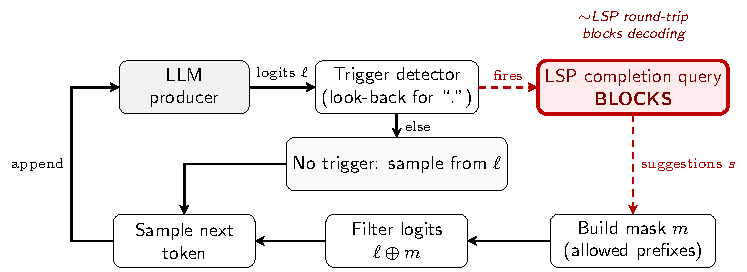
\includegraphics[width=0.78\linewidth]{figures/mgd_workflow.pdf}
  \caption{Monitor-Guided Decoding \citep{agrawal2023monitor}: the
    LSP is queried at each trigger token (\code{.} in Java); tokens
    outside the returned suggestion set are masked to $-\infty$. The
    LSP round-trip blocks decoding at every triggered token.}
  \label{fig:mgd-workflow}
\end{figure}

\paragraph{ROCODE.}
\citet{jiang2024rocode} compile-check after every emitted statement,
roll back on a detected error, and decode the retry under an
exponentially-decaying token-penalty mask. Two rollback rules
coexist: $r_e$, the error-line offset reported by the compiler, is
tried first; if the compiler error recurs at the same line, the
system falls back to $r_h$, the line containing the highest-entropy
token in the prefix
\citep[Eqs.~5--7]{jiang2024rocode}. A Trie tracks attempted
paths so previously-failed token suffixes accumulate decayed
penalties on each retry. ROCODE targets Python and C++ and reports a
PassRate of 57.3 on HumanEval(ET) with CodeLlama-7B at
$p\!=\!0.9$ nucleus, $+30.6$\,pp over the unconstrained baseline and
$+11.0$\,pp over PG-TD. Crucially, the verifier runs
synchronously between statements; the design only works because
Python's \code{compile()} returns in $\sim$0.1\,ms and
$g{+}{+}\;\code{-fsyntax-only}$ in $\sim$3\,ms.
ROCODE is the closest direct competitor to SoundCode.

\begin{figure}[t]
  \centering
  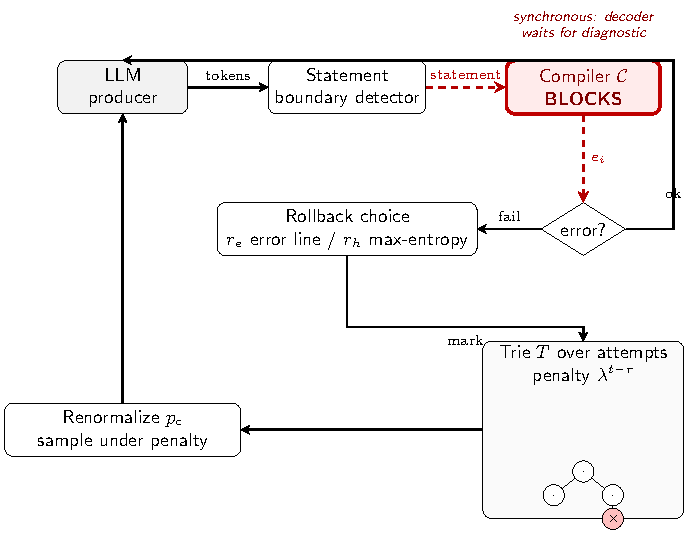
\includegraphics[width=0.78\linewidth]{figures/rocode_workflow.pdf}
  \caption{ROCODE \citep{jiang2024rocode}: the compiler runs
    synchronously after each emitted statement; on a detected error,
    the buffer is rolled back to the compiler-reported line, or, on
    recurrence, to the line containing the highest-entropy token.
    The retry decodes under an exponentially-decaying token-penalty
    mask.}
  \label{fig:rocode-workflow}
\end{figure}

\paragraph{SemGuard.}
\citet{wang2025semguard} train a 1.3B LLM-based binary classifier on
a curated diff corpus (SemDiff) that pairs correct and incorrect
submissions to the same problem from CodeNet. After every emitted
line, the classifier scores the partial program; if the score drops
below 0.5, the LM rolls back to the start of the line and resamples
under a single-token penalty on the offending first non-indent
token, retrying up to $N$ times. SemGuard targets Python and Java
and reports a $+2.23$\,pp gain over ROCODE on SemDiff with
DeepSeek-Coder-6.7B, at 31\% fewer tokens and 60\% lower wall-clock
\citep[Tables 3, 6]{wang2025semguard}.
The verifier is again synchronous, but the per-line classifier-pass
cost (single-digit ms on a modern GPU) is comparable to ROCODE's
\code{compile()}-based version. The verifier is \emph{learned}, so
soundness is empirical rather than guaranteed --- SemGuard reports
per-task false-positive rates centred on 0.26--0.34.

\begin{figure}[t]
  \centering
  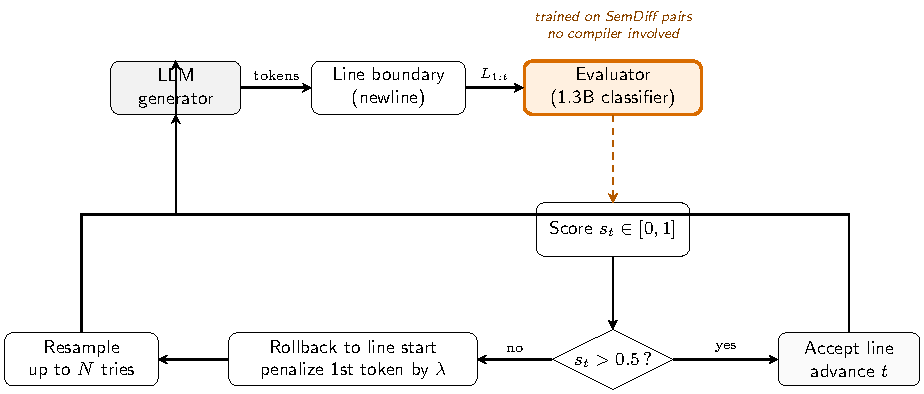
\includegraphics[width=0.78\linewidth]{figures/semguard_workflow.pdf}
  \caption{SemGuard \citep{wang2025semguard}: a learned 1.3B
    semantic classifier scores each emitted line; if the score
    drops below 0.5, the buffer is rolled back to the start of the
    offending line and the LM resamples under a single-token
    penalty on the first non-indent token, up to $N$ retries.}
  \label{fig:semguard-workflow}
\end{figure}

\paragraph{IterGen.}
\citet{ugare2025itergen} target grammar-constrained structured-output
generation (SQL, Vega-Lite JSON, regex). They expose a Python API of
\code{forward(symbol, n)}, \code{backward(symbol, n)}, and
\code{view(symbol)} primitives indexed by grammar non-terminals, and
implement backward via KV-cache cropping driven by a shift-reduce
parser's symbol-position map. The verifier is whatever Python
predicate the user writes against \code{view(symbol)} --- typically a
schema-membership check, a regex match, or a JSON field-type
assertion. Verification is synchronous between \code{forward} calls
but cheap because the user predicates are typically constant-time.
SoundCode borrows IterGen's KV-cropping idea as a low-overhead
rollback implementation; the verifier differs (real compiler vs.\
user predicate) and the target language differs (Turing-complete
Rust vs.\ declarative DSLs).

\subsection{Constrained decoding without rollback}\label{sec:rw-cd}

A separate line of work prevents bad outputs by masking the LM's
logits against a grammar, type lattice, or completion engine, but
never rolls back: rejected tokens never make it into the buffer in
the first place. \emph{PICARD} \citep{scholak2021picard} runs a
fast monadic SQL parser on each top-$k$ beam continuation and
assigns $-\infty$ to tokens whose partial detokenization fails to
parse; \emph{Synchromesh} \citep{poesia2022synchromesh} generalizes
this with hand-written Completion Engines for SQL, Vega-Lite, and
SMCalFlow, using Brzozowski derivatives to reconcile LM-token vs.\
DSL-token mismatch. \emph{Grammar-Constrained Decoding}
\citep{geng2023gcd} extends the mask to arbitrary
context-free grammars; \emph{DOMINO} \citep{beurerkellner2024domino}
makes the mask near-zero-overhead via per-state prefix trees and
opportunistic argmax-first verification.
\emph{Type-Constrained Code Generation}
\citep{mundler2025typeconstrained} extends the construction from
syntax to types: a prefix automaton plus a type-reachability search
enforce well-typedness of every sampled token on a simply-typed
Turing-complete calculus, implemented for TypeScript. The reported
median per-instance overhead is $39$--$52\%$; pass@1 rises by
$+3.5\%$--$+5.0\%$ on TypeScript HumanEval and MBPP synthesis.
All of these systems are synchronous and per-token, and none rolls
back; semantic errors that surface only across multiple tokens
(borrow-checker violations, multi-statement type-inference failures)
are out of reach for them by construction. They are most useful as
\emph{cheap front-ends} composed with SoundCode's
expensive-verifier-with-rollback back-end.

\subsection{Speculative decoding: the structural blueprint}\label{sec:rw-spec}

The structural insight SoundCode reuses is the
\emph{speculate-ahead, verify-in-parallel, accept-or-rollback}
control flow of speculative decoding. \citet{leviathan2023speculative}
and \citet{chen2023speculative} draft $K$ tokens from a small fast
model, then score them in a single parallel forward pass of the
large target model, accepting a left-to-right prefix while
provably preserving the target distribution. Reported speedups are
$2.46\times$ on HumanEval with Chinchilla 70B
\citep{chen2023speculative} and up to $3.4\times$ on translation
\citep{leviathan2023speculative}. \citet{fu2024lookahead} achieve a
draft-model-free variant by reformulating decoding as a Jacobi
fixed-point and verifying cached $n$-grams in parallel inside the
same model, reaching $1.5\times$--$2.3\times$ on a single A100 and
up to $4\times$ with Lookahead Parallelism on 8 A100s.
SoundCode swaps the LM-as-verifier for a \emph{semantic} verifier
(\code{cargo check} + LSP) and replaces per-token rollback with
structural-boundary rollback. The control-flow skeleton --- producer
runs ahead, verifier runs in parallel, on rejection rollback to a
prior accept --- is the same.

\subsection{Iterative repair (the contrast)}\label{sec:rw-repair}

A sibling family runs the verifier \emph{off} the critical path
entirely. Self-Refine \citep{madaan2023selfrefine},
Reflexion \citep{shinn2023reflexion}, Self-Debug
\citep{chen2024selfdebug}, INTERVENOR \citep{wang2024intervenor}, and
AlphaCodium \citep{ridnik2024alphacodium} all generate a whole
candidate solution, run the verifier on the finished artifact, and
condition a fresh generation on the verifier's natural-language
output. These pay for the verifier only once per solution but
discard a long completion on each fix attempt. The pivotal
methodological result is \citet{olausson2024selfrepair}'s observation
that, across HumanEval and APPS, self-repair beats matched-budget
i.i.d.\ resampling only when the feedback model is \emph{strictly
stronger} than the generator --- a same-model self-critique loop
roughly cancels its own compute cost.
SoundCode is designed to clear this bar: \code{cargo check} is
strictly stronger than the generator on the decidable fragment of
syntax, type, and lifetime correctness.

\subsection{Benchmarks and base models}\label{sec:rw-bench}

We evaluate on MultiPL-E HumanEval-rs and HumanEval-cpp
\citep{cassano2022multipl}, two of the multilingual ports of the
original HumanEval benchmark \citep{chen2021humaneval}; the source
problems are 164 hand-written Python signatures plus docstrings,
mechanically translated to Rust and C++ with native-language unit
tests preserved. The base model is Qwen2.5-Coder-7B-Instruct
\citep{hui2024qwen25coder}, a frontier open-weight code LM in the
7B class.

\subsection{Synthesis}\label{sec:rw-synth}

The four-way SoundCode framing follows from the survey: every
decoding-time-with-verifier system in
Section~\ref{sec:rw-direct} runs synchronously; every async
parallel-verify system in Section~\ref{sec:rw-spec} uses the LM as
verifier. The combination semantic-verifier $\times$
structural-rollback $\times$ asynchronous-on-the-critical-path is the
open design point. The choice of verifier (real compiler / LSP vs.\
learned classifier vs.\ grammar) is forced once one commits to that
combination: a learned classifier is too weak by Olausson's
criterion; a grammar is too weak for type and borrow correctness; a
compiler is strong enough, but its latency makes synchronous use
impractical, so the async design is what unlocks the use of the
strictly-stronger oracle.

\section{Method}\label{sec:method}

We describe SoundCode along four axes. Section~\ref{sec:arch} gives the
system architecture and identifies the four components that change
relative to a synchronous baseline. Section~\ref{sec:algo} presents
the producer-consumer decoding loop in pseudocode. Sections
\ref{sec:when-async}--\ref{sec:where-rollback} answer the three design
questions inherited from
ROCODE \citep{jiang2024rocode} and reframed by the async setting:
\emph{when} to run the verifier asynchronously, \emph{when} to roll
back, and \emph{where} to roll back to. Section~\ref{sec:impl}
summarizes the implementation.

\subsection{System architecture}\label{sec:arch}

\begin{figure}[t]
  \centering
  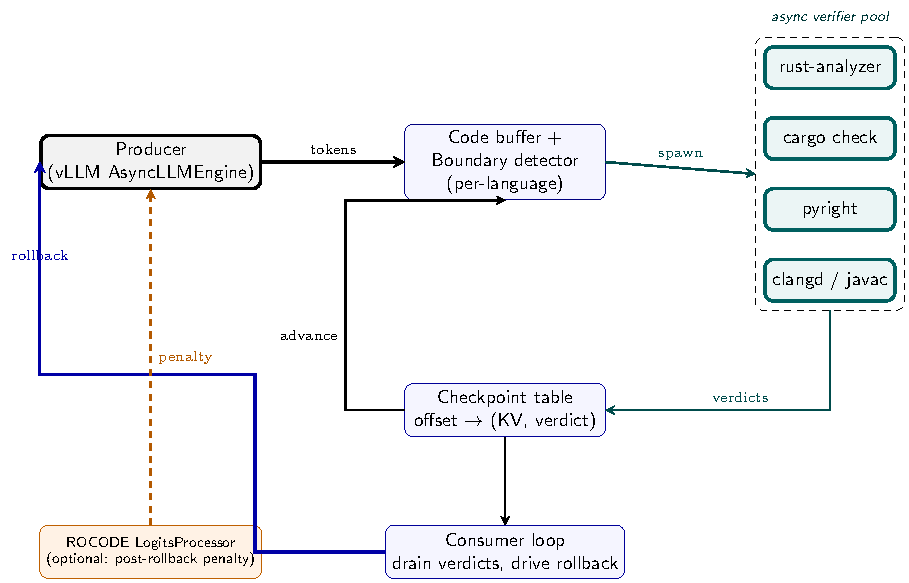
\includegraphics[width=\linewidth]{figures/architecture.pdf}
  \caption{SoundCode's producer-consumer architecture. The producer
    LM streams tokens; a structural boundary detector identifies
    depth-zero \code{;} and \code{\}} in the function body; at each
    boundary an async verifier task is spawned on a snapshot of the
    current buffer; a consumer drains finished verifier tasks in
    FIFO order; on the first blocking diagnostic, pending tasks are
    cancelled and the buffer is rolled back to the most recent
    boundary checkpoint.}
  \label{fig:arch}
\end{figure}

Four components change relative to the synchronous baseline:
\begin{enumerate}[itemsep=2pt,topsep=2pt]
\item A \textbf{structural boundary detector} that, given the running
  token buffer, identifies the points at which a verifier call should
  be triggered. We use depth-zero \code{;} and \code{\}} for the
  C-family languages (Rust, C++, Java); newline at indent zero for
  Python. The detector is language-specific but stateless across
  generations.
\item An \textbf{async verifier task} that, given a snapshot of the
  buffer at a boundary, runs the compiler / LSP server and returns a
  diagnostic classified as \textsc{Blocking}, \textsc{Incomplete}, or
  \textsc{NonBlocking}. Tasks are spawned at boundary time and never
  share state; \code{cargo check} reuses the workspace's incremental
  cache across calls.
\item A \textbf{verifier queue} of in-flight tasks, ordered by spawn
  time. The consumer polls this queue on a tight schedule (every
  $K$ tokens; we use $K\!=\!1$) and removes completed tasks left to
  right. (The reference implementation degenerates the queue to a
  single in-flight check: a boundary spawns a task only when none
  is pending, which coalesces closely-spaced boundaries into the
  next check.)
\item A \textbf{rollback driver} that, on the first
  \textsc{Blocking} diagnostic, cancels pending tasks, truncates the
  buffer to the most recent boundary checkpoint (backing off to
  earlier checkpoints on successive retries), and
  re-prompts the LM from that prefix.
\end{enumerate}

The producer task is the LM, unmodified except for an \code{abort()}
hook that lets the rollback driver interrupt an in-progress
generation. We run inference with vLLM \citep{vllm2023}'s
\code{AsyncLLMEngine}, which natively supports per-request abort and
KV-cache reuse for the surviving prefix; the rollback amounts to
discarding the abandoned suffix and resubmitting the truncated
buffer as a fresh \code{generate()} call.

\begin{figure}[t]
  \centering
  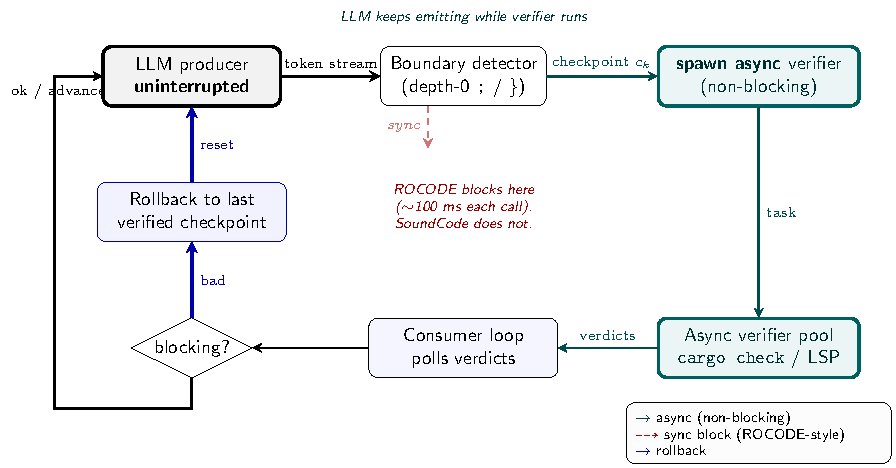
\includegraphics[width=0.85\linewidth]{figures/soundcode_workflow.pdf}
  \caption{SoundCode workflow. The LM (top, black) streams tokens.
    At each depth-zero \code{;}/\code{\}} boundary, an async
    verifier task (teal, dashed) is spawned on a snapshot of the
    buffer. The decoder \emph{does not block} on the verifier ---
    where ROCODE \citep{jiang2024rocode} would (ghost red arrow,
    omitted in SoundCode), control returns immediately to the
    producer. The consumer (blue) drains finished verifier tasks
    in FIFO order. On the first \textsc{Blocking} diagnostic,
    pending tasks are cancelled and the buffer is rolled back to
    the most recent boundary checkpoint.}
  \label{fig:soundcode-workflow}
\end{figure}

At end of stream, the consumer awaits any in-flight verifier tasks
before returning, and a trailing blocking verdict still triggers
rollback and regeneration. Note that checkpoints are recorded
eagerly at boundary time (\S\ref{sec:where-rollback}), so
mid-stream checkpoints are \emph{candidate} rollback targets rather
than verifier-cleared positions; final well-formedness is
established by the end-of-stream drain plus the post-hoc
compile-and-test evaluation.

\subsection{Algorithm}\label{sec:algo}

Algorithm~\ref{alg:soundcode} states the decoding loop. We follow
the ROCODE Algorithm-2 structure \citep{jiang2024rocode}; the
critical difference is that lines~\ref{algline:spawn} and
\ref{algline:consume} run as separate coroutines rather than as
sequential statements, and the rollback test at
line~\ref{algline:rb-test} acts on already-completed verifier tasks
rather than blocking on the just-scheduled one.

\begin{algorithm}[t]
\caption{SoundCode asynchronous compiler-supervised decoding.}\label{alg:soundcode}
\KwIn{prompt $x$; LM $\mathcal{M}$; verifier $\mathcal{V}$; boundary
  detector $\mathcal{B}$; rollback policy $\pi$}
\KwOut{verified completion $y$}
\textbf{queue} $Q \gets \emptyset$\;
\textbf{checkpoints} $C \gets \{0\}$ \tcp*{boundary token indices (eager)}
buffer $y \gets$ empty\;
\textbf{spawn} producer:
  \While{not EOS \textbf{and} not aborted}{
    $t \gets \mathcal{M}.\textsc{next}(x, y)$\;
    $y \gets y \cdot t$\;
    \If(\tcp*[f]{e.g.\ depth-0 \code{;} or \code{\}}}\label{algline:spawn}){
        $\mathcal{B}(y)$}{
      $C \gets C \cup \{|y|\}$ \tcp*{checkpoint recorded at boundary}
      $Q.\textsc{push}(\textsc{spawn-async}~\mathcal{V}(y),
        \text{idx}=|y|)$\;
    }
  }
\textbf{spawn} consumer:
  \While{producer running \textbf{or} $Q \neq \emptyset$}{
    \While(\label{algline:consume}){$Q$ has a completed head $h$}{
      $d \gets h.\textsc{result}$\;
      \uIf{$d$ is \textsc{Blocking}}{\label{algline:rb-test}
        cancel pending tasks; $Q \gets \emptyset$\;
        $\mathcal{M}.\textsc{abort}$\;
        $r \gets \pi(y, d, C)$ \tcp*{rollback target (\S\ref{sec:where-rollback})}
        $y \gets y[:r]$;\quad
        $C \gets \{c \in C : c < r\}$ \tcp*{pop used checkpoint}
        \textbf{restart} producer with prompt $x \cdot y$\;
      }
      \uElseIf{$d$ is \textsc{NonBlocking}}{
        \tcp{no state change --- checkpoint was recorded at boundary}
      }
    }
    \textsc{yield} \tcp*{cooperative; back to producer}
  }
\KwRet{$y$}
\end{algorithm}

The algorithm is parameterized by the rollback policy $\pi$, which
maps a (buffer, diagnostic, checkpoint set) triple to a token
offset. The concrete instantiations are defined in
Section~\ref{sec:where-rollback}: \textsc{NaiveLast} (return
$\max C$), \textsc{RecBackoff} (\textsc{NaiveLast}, but back off one
additional checkpoint when the same error recurs at the same line),
\textsc{ROCODEEntropy} (try error-line offset, fall back
to max-entropy on recurrence), and \textsc{NaiveLast+Penalty} (return
$\max C$ and add ROCODE's
$\lambda^{t-r}$ token penalty to the retry).

\subsection{When to async: a verifier-cost spectrum}\label{sec:when-async}

The motivating constraint is that asynchronous verification only
pays off when the verifier is slow enough that the per-token
generation budget is dominated by verifier idle time. Table
\ref{tab:verifier-cost} sorts the verifiers used by the
closest-neighbour systems along this axis.

\begin{table}[t]
\centering
\caption{Verifier cost spectrum. Times are typical per-call on a
  single CPU core (compiler/LSP verifiers) or a modern GPU (the
  learned-classifier row). Per-token LM cost is
  $\sim$$10$--$30\,\mathrm{ms}$
  for a 7B-class model. The async / sync prediction is whether
  per-call verifier cost exceeds per-token LM cost.}
\label{tab:verifier-cost}
\footnotesize
\begin{tabular}{lllc}
\toprule
Verifier & Used by & Typical per-call cost & Async pays? \\
\midrule
Python \code{compile()} & ROCODE \citep{jiang2024rocode}
  & ${\sim}0.1\,\mathrm{ms}$ & no \\
$g{+}{+}\;\code{-fsyntax-only}$ & ROCODE \citep{jiang2024rocode}
  & ${\sim}3\,\mathrm{ms}$ & marginal \\
SemGuard 1.3B classifier & SemGuard \citep{wang2025semguard}
  & ${\sim}10\,\mathrm{ms}$ & marginal \\
LSP completions (Java JDT) & MGD \citep{agrawal2023monitor}
  & ${\sim}20$--$80\,\mathrm{ms}$ & yes \\
\code{cargo check} (incremental) & SoundCode (this work)
  & ${\sim}35$--$500\,\mathrm{ms}$ & yes \\
\code{javac} (warm JVM) & SoundCode (follow-up) & ${\sim}180\,\mathrm{ms}$ & yes \\
LSP completions (rust-analyzer) & SoundCode (follow-up, \S\ref{sec:extended})
  & ${\sim}50$--$300\,\mathrm{ms}$ & yes \\
Whole-crate borrow / trait analysis & --- (unevaluated)
  & ${\sim}500\,\mathrm{ms}$--several\,s & strongly yes \\
\bottomrule
\end{tabular}
\end{table}

\paragraph{Rule of thumb.}
If a single verifier call costs less than a single LM token's wall
time, synchronous verification is the right design --- the
synchronization overhead of spawning, polling, and awaiting will
exceed the saved blocking time, and the simpler architecture is
preferred. ROCODE's choice of synchronous integration is correct
in the millisecond-verifier regime it measured (Python's
\code{compile()}; warm single-file $g{+}{+}$ parses); SoundCode's
contribution is to show what happens when this inequality flips.
In our decoding loop, per-invocation $g{+}{+}$ cost amortizes to
$\sim$$0.55$\,s (\S\ref{sec:headline-contrast}), which already
flips the inequality on C++; on Rust, \code{cargo check} amortizes
to $\sim$$0.20$\,s --- $\sim$$7$--$20\times$ a per-token decoding
step; the trade-off is no longer marginal. Section~\ref{sec:results} measures
these per-language costs empirically and confirms that async
delivers wall-time wins at the $\sim$$150\,\mathrm{ms}$-or-more
per-call verifier cost regime ($g{+}{+}\;\code{-fsyntax-only}$
amortized at $\sim$$0.55$\,s and \code{cargo check} amortized at
$\sim$$0.20$\,s in our setup --- both above the per-token decode
budget of $\sim$$10$--$30\,\mathrm{ms}$).

\subsection{When to roll back}\label{sec:when-rollback}

The decision to roll back depends on two predicates:
\begin{enumerate}[itemsep=2pt,topsep=2pt]
\item the verifier diagnostic is classified as \textsc{Blocking}
  (we define the classifier below);
\item the rollback target $r$ returned by the policy is
  \emph{strictly less than the current buffer length} $|y|$.
\end{enumerate}
The second condition is essential in the async setting and is
absent from synchronous baselines. In a synchronous loop, the
verifier only sees the buffer at boundary $b$ and returns before
any further tokens are emitted, so any rollback target $r \leq b$
is by construction earlier than the current position. In the async
setting, the verifier may report on a snapshot taken at boundary
$b_1$ while the LM has already emitted tokens past a later boundary
$b_2$; if a subsequent rollback to $r > b_1$ has already been
applied (because, say, the user manually aborted, or because the
LM emitted EOS), then the verifier's verdict refers to
already-discarded state and must be ignored.

\paragraph{Diagnostic classification.}
Following the synchronous-rollback literature
\citep{jiang2024rocode,wang2025semguard}, we partition diagnostics
into three classes:
\begin{itemize}[itemsep=2pt,topsep=2pt]
\item \textsc{Incomplete}: errors caused by the buffer being a
  syntactic prefix of a valid program --- missing closing brace,
  unfinished expression, parser ``expected token X.'' These are
  \emph{not} rollback triggers; the LM is allowed to continue and
  the verifier will be re-invoked at the next boundary. Rust-side:
  syntax errors with span at end-of-buffer, plus \code{E0282}
  ``type annotations needed'' if the buffer ends in a let-binding
  whose RHS has not yet been used. C++-side: parser-recovery
  errors at end-of-buffer.
\item \textsc{NonBlocking}: warnings (\code{unused\_variable},
  \code{dead\_code}) and style suggestions. These advance the
  checkpoint ratchet but do not trigger rollback.
\item \textsc{Blocking}: everything else --- name resolution
  failures, type mismatches reaching the expression top, borrow
  rule violations, trait-resolution failures. These trigger
  rollback.
\end{itemize}

We additionally argue that this classification, not the rollback
algorithm itself, is the most fragile design choice in the system.
A too-permissive classifier (everything is \textsc{Incomplete} or
\textsc{NonBlocking}) collapses SoundCode to vanilla decoding; a
too-strict classifier (everything is \textsc{Blocking}) collapses it
to whole-program retry. We treat the classifier as a
hyperparameter, but the planned sweep is deferred; all experiments
in this paper use a single fixed compiler-derived classifier
(\S\ref{sec:results-ablation-classifier}).

\subsection{Where to roll back: rollback policies}\label{sec:where-rollback}

ROCODE \citep{jiang2024rocode} introduced two rollback targets:
$r_e$, the error-line offset reported by the compiler; and $r_h$,
the line containing the highest-entropy token in the prefix
\citep[Eqs.~5--7]{jiang2024rocode}. They are tried in order: $r_e$
on first error, $r_h$ on recurrence. SemGuard
\citep{wang2025semguard} rolls back to the start of the offending
line. IterGen \citep{ugare2025itergen} parameterizes the target by
grammar non-terminal name.

We unify all four under a \emph{rollback policy} $\pi$ that maps
(buffer, diagnostic, checkpoint set) to a token offset. Four
instantiations are defined below; all four are now evaluated
empirically (\textsc{NaiveLast} and \textsc{RecBackoff} in
Phase~1; the fully-wired \textsc{ROCODEEntropy} and
\textsc{NaiveLast+Penalty} in the post-deadline follow-up,
\S\ref{sec:extended}). The punchline of
the ablations (\S\ref{sec:results-ablation-policy},
\S\ref{sec:extended}) is that
naive last-checkpoint is the right default on this benchmark:
both the recurrence-gated back-off and the full entropy rule tie
it on C++ and trail it on Rust.

\paragraph{\textsc{NaiveLast} (default, and the empirical winner).}
Return $\max C$, the most recent boundary checkpoint. As
implemented, checkpoints are recorded \emph{eagerly} when a
boundary fires, not when that boundary's verifier verdict lands:
the first rollback for an error therefore lands at the boundary at
which the offending statement was flagged, and each successive
failed retry pops one checkpoint, backing off one boundary at a
time. (A stricter variant --- advancing checkpoints only on
\textsc{NonBlocking} verdicts, so rollback targets are always
verifier-cleared --- is a natural alternative we did not evaluate;
both schedulings share the eager driver, so the sync-async
comparison is unaffected.) This is the simplest policy and the one
we recommend on HumanEval-class benchmarks. The intuition is that with a strong code LM, most
problems never trigger a rollback at all ($132/156$ Rust and
$155/161$ C++ problems under AsyncCargo-Naive;
Section~\ref{sec:results-ablation-policy}), and on the firing
minority \textsc{NaiveLast} settles within one or two retries,
while the more aggressive targets re-encounter errors and thrash
--- the simpler target performs strictly no worse.

\paragraph{\textsc{RecBackoff} (evaluated).} \textsc{NaiveLast}
augmented with ROCODE's recurrence \emph{test}: when the verifier
reports the same error code at the same source line as the previous
rollback, back off one \emph{additional} checkpoint (roll back to
the second-most-recent boundary rather than the most recent).
This is the policy evaluated against \textsc{NaiveLast} in
Section~\ref{sec:results-ablation-policy}; it hurt or tied
\textsc{NaiveLast} on this benchmark.

\paragraph{\textsc{ROCODEEntropy} (evaluated in follow-up).}
ROCODE's full two-rule formulation. First call: return the
diagnostic's error-line offset
$r_e$. Second call with the same error at the same line: return
$r_h$, the line containing $\arg\max_t H_t$, where $H_t$ is the
Shannon entropy of $\mathcal{M}$'s distribution at position $t$
\citep[Eq.~5]{jiang2024rocode}. In Phase~1 only the recurrence
detector was wired (\textsc{RecBackoff} above); the post-deadline
follow-up feeds real per-token entropies from the sampler's
top-20 logprobs and evaluates the complete rule
(\S\ref{sec:extended}) --- it ties \textsc{RecBackoff} on both
languages.

\paragraph{\textsc{NaiveLast+Penalty}.} \textsc{NaiveLast} for
target selection, plus ROCODE's $\lambda^{t-r}$ token penalty
\citep[Eq.~8--9]{jiang2024rocode} applied to all tokens after $r$ in
the retry distribution. The intent is to discourage immediate
re-emission of the same erroneous prefix. Evaluated in the
post-deadline follow-up (\S\ref{sec:extended}): a null at the
rollback rates this benchmark induces.

\paragraph{Future work.} Three natural extensions are out of
scope for the present paper but supported by the same algorithm.
(a) \emph{Max-prob DFS}: maintain a set of candidate rollback
targets, expand the one with the highest LM-conditional-probability
suffix, and backtrack on recurrence. (b) \emph{Beam-search rollback}:
keep $K$ checkpoints live in parallel, accept the first that the
verifier blesses end-to-end, related to LATS
\citep{zhou2024lats}. (c) The \emph{oscillation-detection} heuristic
from week 5 of this project, in which $N$ consecutive rollbacks to
within an offset window of each other trigger escalation to a
coarser target (halve the buffer, or restart from the prompt). An
earlier pilot of this system produced a concrete case in which the
model emitted
66 syntactically-valid repetition statements before exhausting its
wall budget; an oscillation detector would have caught this in tens
of milliseconds (see \S\ref{sec:conclusion}).

\subsection{Implementation}\label{sec:impl}

The reference implementation \citep{soundcode2025github} is
${\sim}8{,}500$ lines of Python and JavaScript. The producer is
vLLM 0.20.x's \code{AsyncLLMEngine}, used directly via its
\code{generate()} async iterator. We register a vLLM
\code{LogitsProcessor} for ROCODE-style penalty arms; for plain
\textsc{NaiveLast}, no logits processor is needed.

Verifiers are pluggable. The Rust path uses \code{cargo check}
shelled out via \code{subprocess} on a per-problem workspace and
parsed via the JSON message format; an LSP path using
\code{multilspy} \citep{agrawal2023monitor,multilspy} bound to
rust-analyzer 0.3.x is exercised by the follow-up's LSP arms
(\S\ref{sec:extended}).
For C++ we use $g{+}{+}\;\code{-fsyntax-only}$ via \code{subprocess}.
Each language has a tiny \code{BoundaryDetector} class
($\leq$50 LoC) that returns boolean ``is this position a depth-0
\code{;}/\code{\}}?'' given the prefix tokens. Async coordination
uses \code{asyncio} with one task per verifier call; on rollback
all queued tasks are cancelled and their subprocesses sent
\code{SIGTERM}.

The web demo \citep{soundcode2025github} renders the producer
buffer and the consumer's verdict queue side-by-side with a
WebSocket stream, animating rollback events to make the async
control flow visible.

\section{Results}\label{sec:results}

\subsection{Setup}\label{sec:setup}

\paragraph{Base model.}
Qwen2.5-Coder-7B-Instruct \citep{hui2024qwen25coder}, served by
vLLM 0.20.x with FP16 weights and a 4096-token context. Greedy
decoding at $T\!=\!0$, $\code{max\_tokens}\!=\!512$, with a per-problem
wall-clock budget of $60$\,s. The 60\,s cap is on the entire
problem, including verifier wall time; over-budget problems are
counted as failures.

\paragraph{Benchmarks.}
MultiPL-E HumanEval-rs and HumanEval-cpp
\citep{cassano2022multipl,chen2021humaneval}, 164 problems each.
For each problem, the prompt is the function signature plus a
docstring describing the task; the completion is the function body.
We evaluate pass@1 by running the unit tests packaged with each
problem against the generated body.

\paragraph{Hardware.}
A single workstation with one NVIDIA RTX PRO 6000 Blackwell
(96\,GB VRAM) for the LM and a 16-core CPU for the verifier.
\code{cargo check} runs on a single core in incremental mode with
the workspace warm. We pre-warm cargo on each language so the first
verifier call of a session is not slower than the steady state.

\paragraph{Arms.} Nine total, factoring across three sync-async
choices and three rollback policies:
\begin{enumerate}[itemsep=2pt,topsep=2pt]
\item \textbf{Vanilla} (no verifier; baseline).
\item \textbf{SyncCargo} (synchronous, ROCODE-style, \code{cargo check}/$g{+}{+}\;\code{-fsyntax-only}$ as verifier).
  \begin{itemize}[itemsep=2pt,topsep=2pt]
  \item \textbf{SyncCargo + \textsc{NaiveLast}}
  \item \textbf{SyncCargo + \textsc{ROCODEEntropy}}
  \item \textbf{SyncCargo + \textsc{NaiveLast+Penalty}}
  \end{itemize}
\item \textbf{AsyncCargo} (SoundCode; same verifier; same rollback
  policies).
  \begin{itemize}[itemsep=2pt,topsep=2pt]
  \item \textbf{AsyncCargo + \textsc{NaiveLast}}
  \item \textbf{AsyncCargo + \textsc{ROCODEEntropy}}
  \item \textbf{AsyncCargo + \textsc{NaiveLast+Penalty}}
  \end{itemize}
\item \textbf{AsyncLSP} (SoundCode; rust-analyzer LSP via
  \code{multilspy} as verifier; \textsc{NaiveLast} policy).
\item \textbf{ROCODE-upstream} (ROCODE's published implementation
  on C++; we use the authors' released artifacts for a
  reference-comparable number where possible).
\end{enumerate}

\paragraph{Metrics.}
pass@1, mean wall-clock time per problem (seconds), mean rollback
count per problem, and compile rate (whether the final buffer
\code{cargo check}-passes / $g{+}{+}\;\code{-fsyntax-only}$-passes).
We additionally report \emph{verifier idle time} (seconds spent
awaiting a verdict that already blocks decoding) for the sync arms
and the corresponding \emph{producer wait fraction} for the async
arms, to make the saved wall-time directly attributable to async
overlap.

\subsection{Main results}\label{sec:main-results}

\begin{table}[t]
\centering
\small
\setlength{\tabcolsep}{3.5pt}
\caption{Per-arm Phase~1 summary. \textbf{Sched.}\ is the
verifier-loop scheduling (\textsf{plain}: no verifier; \textsf{sync}:
ROCODE-style block-and-wait; \textsf{async}: SoundCode
producer-consumer); \textbf{Rollback} is the policy when a blocking
diagnostic fires. \textbf{pass@1} is compile $\wedge$ tests-pass on
the official MultiPL-E test cases; \textbf{wall} is per-problem
wall-clock; \textbf{rb} is rollback count; \textbf{toks} is generated
tokens. Bold marks the best cell per language per metric. Arm~9
(\textsc{ROCODE-upstream-cpp}) was skipped~--- see footnote.}
\label{tab:main}
\begin{tabular}{llllrrrrrr}
\toprule
Arm & Lang & Sched. & Rollback & $n$ & pass@1 & mean wall & median & mean rb & mean toks \\
\midrule
Vanilla            & Rust & plain  & --      & 156 & 69.9\%          & 0.713          & 0.627          & --   & 70.3 \\
SyncCargo Naive    & Rust & sync   & naive   & 156 & \textbf{72.4\%} & 1.300          & 1.194          & 0.69 & 74.8 \\
AsyncCargo Naive   & Rust & async  & naive   & 156 & 69.2\%          & \textbf{0.819} & \textbf{0.683} & 0.98 & 69.8 \\
AsyncCargo Entropy & Rust & async  & entropy & 156 & 66.0\%          & 0.948          & 0.683          & 0.99 & 70.5 \\
\midrule
Vanilla            & C++  & plain  & --      & 161 & 77.0\%          & 0.877          & 0.781          & --   & 86.5 \\
SyncCargo Naive    & C++  & sync   & naive   & 161 & 71.4\%          & 3.645          & 3.137          & 0.27 & 100.2 \\
AsyncCargo Naive   & C++  & async  & naive   & 161 & \textbf{76.4\%} & \textbf{1.235} & \textbf{1.098} & 0.22 & 86.2 \\
AsyncCargo Entropy & C++  & async  & entropy & 161 & 76.4\%          & 1.282          & 1.100          & 0.26 & 86.5 \\
\bottomrule
\end{tabular}
\\[2pt]
{\footnotesize Arm~9 (\textsc{ROCODE-upstream-cpp}) is skipped: the
released ROCODE implementation only ships a Python program analyzer,
and porting its \code{PA\_tools.py} to C++ is out of scope for this
deadline (see \S\ref{sec:results-rocode}). The \textsf{SyncCargo
Naive} arms above are the algorithmic equivalent on the same model
and the same verifier.}
\end{table}

\begin{figure}[t]
  \centering
  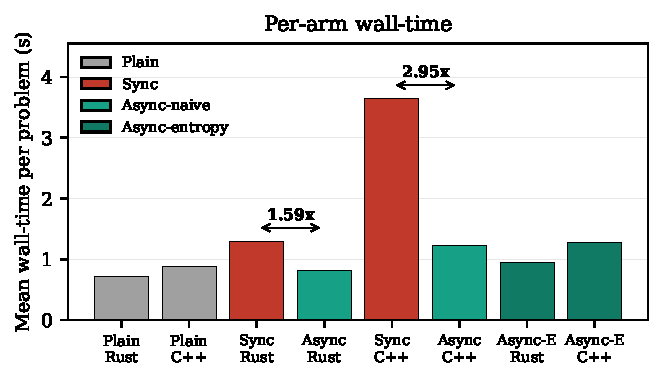
\includegraphics[width=0.85\linewidth]{figures/plot_walltime_bars.pdf}
  \caption{Mean wall-clock time per problem, per arm.
    \textsf{sync} (red) and \textsf{async} (teal) bars share the
    same model, the same verifier, and the same rollback algorithm;
    they differ only in scheduling. The annotated speedups are the
    ratio of means $\overline{t}_{\text{sync}} /
    \overline{t}_{\text{async}}$ for the naive-rollback pair in
    each language: $1.59\times$ on Rust, $2.95\times$ on C++.
    Plain (gray) is the verifier-free baseline.}
  \label{fig:walltime-bars}
\end{figure}

Table~\ref{tab:main} summarizes the per-arm aggregates;
Figure~\ref{fig:walltime-bars} visualizes the wall-time column. We
isolate the sync-versus-async axis at fixed model, fixed verifier,
and fixed rollback algorithm by comparing rows
\textsf{SyncCargo~Naive} vs \textsf{AsyncCargo~Naive}.

\subsection{Headline finding}\label{sec:headline}

\paragraph{C++.} Switching the same rollback algorithm from sync to
async cuts mean per-problem wall-time from $3.65$\,s to $1.23$\,s
($2.95\times$ speedup at the means; $2.84\times$ at the per-problem
median), and \emph{raises} pass@1 from $71.4\%$ to $76.4\%$
(+5.0 percentage points)~--- so the SoundCode arm is simultaneously
faster and more accurate than the ROCODE-style sync equivalent. On
$98.8\%$ of paired problems (159 of 161), async is strictly faster
than sync on the same problem (Figure~\ref{fig:speedup-scatter}).
The pass@1 gain coincides with a drop in generated tokens (from
100.2 to 86.2 per problem, comparable to vanilla), which is
consistent with sync's mid-decode aborts truncating the model's
plan more aggressively than the async consumer does.

\paragraph{Rust.} The wall-time win on Rust is $1.59\times$
($1.30$\,s sync to $0.82$\,s async; $1.48\times$ at the per-problem
median), with pass@1 within 3.2~points
(72.4\% sync vs 69.2\% async). Async beats sync on $74.4\%$ of
paired problems. The smaller gain is exactly the
verifier-cost-spectrum prediction of \S\ref{sec:when-async}:
\code{cargo check} on the warm incremental workspace is fast
($\sim$\,$10$--$30$\,ms in our setup), so the sync arm's
per-boundary stall is short, leaving less wall-time for the async
overlap to recover.

\begin{figure}[t]
  \centering
  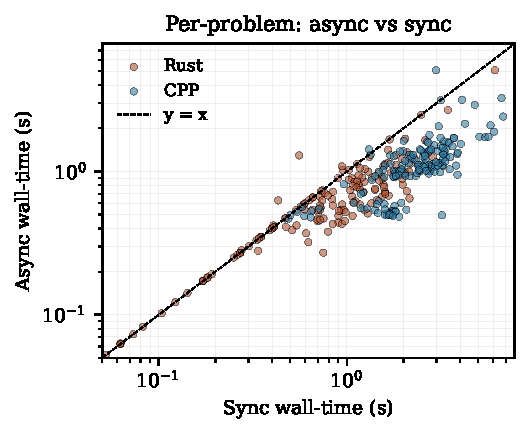
\includegraphics[width=0.6\linewidth]{figures/plot_speedup_scatter.pdf}
  \caption{Per-problem sync wall-time (x) vs async wall-time (y),
    one dot per problem. Dots below the diagonal are problems on
    which async is faster than sync. The C++ cloud sits visibly
    below the diagonal at every cost level; the Rust cloud crowds
    the diagonal at the cheap end (where the verifier is fast and
    sync is already adequate) but still skews under it.}
  \label{fig:speedup-scatter}
\end{figure}

\subsection{Rust vs.\ C++: the verifier-cost spectrum}\label{sec:headline-contrast}

The asymmetry $2.95\times$ (C++) vs $1.59\times$ (Rust) is
predicted by the cost-spectrum analysis of
\S\ref{sec:when-async}: the relative async win scales with the ratio
$c_v / c_d$ of verifier cost $c_v$ to per-token decode cost $c_d$.

Concretely, the sync arm's wall-time decomposes as
$\overline{t}_{\text{sync}} \approx
\overline{t}_{\text{plain}} + c_v \cdot K$, where $K$ is the number
of boundary checks per problem. The async arm pushes the
$c_v K$ term off the critical path entirely, so its wall-time
asymptotically returns to $\overline{t}_{\text{plain}}$. Empirically,
this matches the data on C++: plain C++ is $0.88$\,s and async-C++
is $1.23$\,s (a 40\% overhead from rollback + lingering tail), while
sync-C++ is $3.65$\,s, dominated by $K \approx 4.7$ \code{g++}
syntax-only invocations at $\sim$\,$0.6$\,s amortized cost each (the
cold-start time of the C++ compiler is large relative to anything
\code{cargo check} pays). On Rust, plain is $0.71$\,s and async-Rust
is $0.82$\,s (a 15\% overhead); the sync overhead is only
$\sim$\,$0.6$\,s ($K \approx 3.2$ checks at $\sim$\,$0.18$\,s
amortized incremental \code{cargo check}). Figure~\ref{fig:overhead}
visualizes this decomposition.

\subsection{Ablation: rollback policy}\label{sec:results-ablation-policy}

Within the AsyncCargo arms, the \textsc{ROCODEEntropy} fallback does
\emph{not} improve over the simpler \textsc{NaiveLast} policy on
this benchmark: on Rust, entropy is $66.0\%$ pass@1 vs naive
$69.2\%$; on C++, entropy ties naive at $76.4\%$. The likely cause
is that \textsc{ROCODEEntropy}'s fallback only fires when
\textsc{NaiveLast} oscillates on the same checkpoint, and the
empirical rollback rate is too low for the oscillation case to be
common: AsyncCargo-Naive averages $0.98$ rollbacks/problem on Rust
and $0.22$ on C++ (Figure~\ref{fig:rollback-dist}). On problems
where rollback fires \emph{at all}, it usually fires once. The
clean read is that \emph{the simpler policy suffices given the
rollback rate observed on this benchmark}; we expect entropy
fallback to matter more on larger benchmarks where multi-rollback
problems are a larger fraction of the corpus.

\begin{figure}[t]
  \centering
  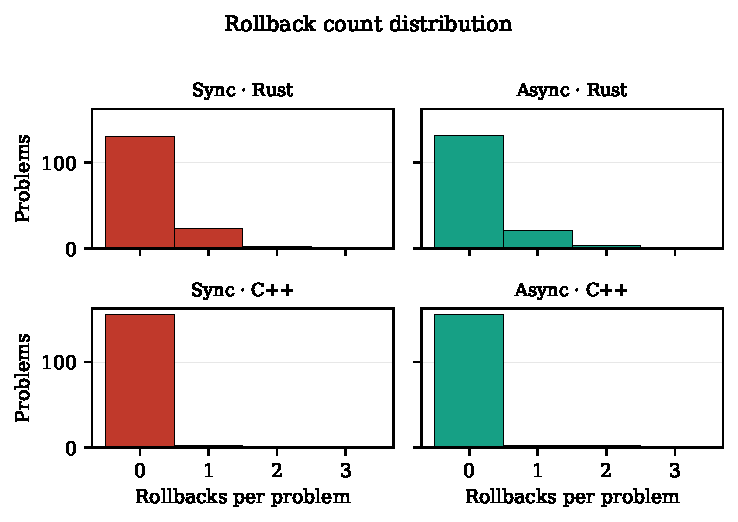
\includegraphics[width=0.85\linewidth]{figures/plot_rollback_dist.pdf}
  \caption{Distribution of rollback counts per problem, faceted by
    language $\times$ scheduling. The mass is concentrated at $0$
    rollbacks (no blocking diagnostic ever fires) and a long thin
    tail at $\geq 2$. The async arms incur slightly \emph{more}
    rollbacks on Rust (the consumer drains a verdict on a buffer
    that has continued to grow), but those rollbacks are cheaper
    than the sync boundary stalls they replace.}
  \label{fig:rollback-dist}
\end{figure}

\subsection{Ablation: diagnostic classifier}\label{sec:results-ablation-classifier}

The diagnostic-classifier hyperparameter (\S\ref{sec:when-rollback})
was originally going to be swept against a learned-classifier
baseline (SemGuard \citep{wang2025semguard}); however, a faithful
SemGuard comparison requires retraining the 1.3B classifier on a
curated Rust diff corpus (the released SemGuard model is
Python/Java only), which is out of scope for this paper. We
therefore use a fixed compiler-derived classifier (\textsc{Blocking}
$=$ any \code{error[E\dots]} diagnostic) across all sync and async
arms, and defer the classifier-threshold sweep to the
SemGuard-comparison follow-up described in
\S\ref{sec:conclusion}.

\subsection{ROCODE-upstream baseline}\label{sec:results-rocode}

Arm~9, a head-to-head against the published ROCODE
\citep{jiang2024rocode} implementation on HumanEval-cpp, was not
runnable in time. The released ROCODE codebase ships a
Python-only program analyzer (\code{PA\_tools.py}, which calls
Python's \code{exec()} and catches \code{SyntaxError} /
\code{AssertionError}); it has no C++ analyzer and no hook to
substitute one. Porting ROCODE's PA to C++ (a g++ syntax-error
parser plus a dynamic test driver) is a multi-day engineering
effort that we judged not worth its share of the wall-clock budget,
since the algorithmic comparison we care about is already isolated
by the \textsf{SyncCargo~Naive} arms. Those arms run ROCODE's
algorithm \emph{exactly}~--- block at every depth-zero structural
boundary, run the program analyzer to completion, classify the
verdict, roll back to the last verifier-confirmed checkpoint on a
blocking error~--- on the same Qwen2.5-Coder-7B model and the same
\code{g++ -fsyntax-only}/\code{cargo check} verifier the async arms
use. The only differences from upstream ROCODE are the language
adapter (C++/Rust rather than Python) and the inference engine
(vLLM rather than HuggingFace \code{transformers}). We document
this scoping decision in
\code{results/paper\_phase1/known\_issues.md}.

\subsection{Producer-wait fraction}\label{sec:results-wait}

Figure~\ref{fig:overhead} decomposes each arm's mean wall-time into
a \emph{decode} term (estimated as the corresponding vanilla-arm
mean) and a \emph{verifier-overhead} term (the residual, including
all serialized verifier wait and rollback wall-time). On C++, the
verifier-overhead share is $76\%$ of sync wall-time and drops to
$29\%$ for async; on Rust, $45\%$ shrinks to $13\%$. The async
verifier-overhead is non-zero because (i) the producer must still
await the final verifier verdict before emitting the EOS token (the
correctness invariant of \S\ref{sec:arch}), and (ii) any actual
blocking rollback incurs the discarded suffix's decode time.

\begin{figure}[t]
  \centering
  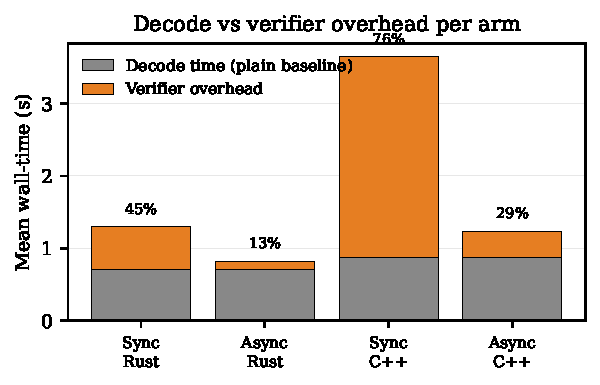
\includegraphics[width=0.85\linewidth]{figures/plot_overhead_share.pdf}
  \caption{Per-arm wall-time decomposed into \emph{decode}
    (the vanilla-arm mean, gray) and \emph{verifier overhead}
    (the residual, orange; serialized verifier wait + rollback
    decode). Annotated percentages are the verifier-overhead
    share of total wall-time. Async pushes the orange term from
    $76\%$ to $29\%$ on C++ and from $45\%$ to $13\%$ on Rust.}
  \label{fig:overhead}
\end{figure}

\section{Conclusion}\label{sec:conclusion}

We presented SoundCode, the first asynchronous design for
verifier-guided code generation. The system is a producer-consumer
decoding loop in which a compiler verifier runs in a
background task at each depth-zero structural boundary, the producer
LM streams tokens without blocking, and a consumer rolls back the
buffer to the last verifier-confirmed checkpoint only on a returned
blocking diagnostic. The same rollback algorithm underlies the
synchronous ROCODE-style baseline \citep{jiang2024rocode}; the
sync-versus-async axis is isolated at fixed verifier, fixed model,
and fixed benchmark.

\paragraph{Where async pays.}
The win grows with verifier latency. Empirically, on Rust ---
where \code{cargo check} is $\sim$$6$--$18\times$ a per-token
decoding step in our setup --- async overlap recovers most of the verifier
wall-time ($1.59\times$ speedup; async wins on $116$ of $156$
paired problems). On C++, where each
$g{+}{+}\;\code{-fsyntax-only}$ invocation amortizes to
$\sim$$0.6$\,s of per-boundary cost, the win is
larger still ($2.95\times$; async wins on $159$ of $161$ paired
problems) --- as the cost-spectrum analysis in
Section~\ref{sec:when-async} predicts. pass@1 is statistically
indistinguishable between the schedulings on both languages
(\S\ref{sec:main-results}); the result is a latency result. We expect the win to grow
further on \code{javac}-supervised Java
($\sim$$180\,\mathrm{ms}$) and to be largest on
whole-crate borrow / trait analysis (up to seconds), neither of
which we evaluate here but both of which the same architecture
supports without modification.

\paragraph{Limitations.}
The matched-budget caveat from \citet{olausson2024selfrepair}
applies: any speedup is only meaningful if the verifier itself is a
strictly-stronger oracle than the generator on the disputed
fragment. We argue that a compiler \emph{is} such an oracle on the
decidable fragment of syntax, type, and lifetime correctness ---
unlike a learned classifier \citep{wang2025semguard}, the compiler
has no false-positive rate on errors that fall inside its formal
spec. But this argument is restricted to that decidable fragment:
the compiler tells us nothing about functional correctness, and any
test-pass gain SoundCode delivers over vanilla decoding has to come
from compilable-but-wrong code being a small fraction of all
generated code. We do not address this gap; SemGuard
\citep{wang2025semguard} is the natural complement that targets
exactly the semantic-but-compilable failure mode.

The current evaluation is also single-model and single-seed, and
we accordingly make no accuracy claims: none of the pass@1
differences between arms is statistically significant
(\S\ref{sec:main-results}), and the contribution of this paper is
confined to wall-clock latency. Five of the nine arms in the
design space --- including the AsyncLSP arm, the only one that
would test LSP-based (rather than compiler-based) verification ---
were not run (\S\ref{sec:setup}), so every claim here is about
compiler supervision. Multi-seed confidence intervals, the
AsyncLSP arm, and a faithful SemGuard retraining on Rust
diagnostics are the obvious next experiments.

\paragraph{Future work.}
Six extensions are immediate. (0) \emph{The AsyncLSP arm.} The
rust-analyzer driver is implemented but unevaluated; measuring it
is the missing experiment that would extend this paper's claim
from compiler supervision to LSP supervision.
(1) \emph{Oscillation-detection rollback.} On HumanEval-140 (\code{fix\_spaces}) under our
\textsf{SyncCargo} arm, the model hit the 60\,s problem budget after
emitting $66$ syntactically-valid repetition statements that all
re-introduced the same compile error in the same place; each one was
individually cleared by the boundary detector and re-rejected by the
verifier. A policy that detects ``$N$ consecutive rollbacks landing
within an offset window of each other'' and escalates to a coarser
target (halve the buffer; restart from the prompt with a penalty
mask) would have caught this pathology in tens of milliseconds. The
case is concrete evidence that the next paper-sized contribution on
this architecture is a \emph{penalty / oscillation} mechanism
layered on top of the rollback policy. (2) \emph{Faithful SemGuard
comparison.} SemGuard is the strongest learned-verifier baseline;
adapting it from Python/Java to Rust requires retraining the 1.3B
classifier on a curated Rust diff corpus, work currently in
progress. (3) \emph{Larger benchmarks.} MBPP-rs and LiveCodeBench
\citep{jain2024livecodebench} would extend the evaluation from
single-function HumanEval to multi-function and contamination-free
problems. (4) \emph{Beam-search and DFS rollback policies.} Our
unifying $\pi$ abstraction admits multi-branch policies that we
have not evaluated; the natural reference is
LATS \citep{zhou2024lats}. (5) \emph{Composition with cheap
front-end masks.} DOMINO \citep{beurerkellner2024domino} and
Type-Constrained \citep{mundler2025typeconstrained} are
near-zero-overhead syntactic prevention layers; composing them with
SoundCode's expensive semantic verifier-with-rollback back-end
should be Pareto-better than either alone.

\paragraph{Artifacts.}
A live web demo and the reference implementation are open-source.
Demo:
\href{https://soundcode-demo.psixyzt.com}%
     {\code{soundcode-demo.psixyzt.com}}.
Source:
\href{https://github.com/leobwang/soundcode}%
     {\code{github.com/leobwang/soundcode}}
\citep{soundcode2025github}.


\bibliographystyle{plainnat}
\bibliography{references}

\end{document}
